\documentclass[tikz,border=6pt]{standalone}
\usepackage[T1]{fontenc}
\usepackage[utf8]{inputenc}
\usepackage{amsmath,amssymb}
\usepackage{graphicx}
\usepackage{xcolor}
\usepackage{tikz}
\usepackage{pgfplots}
\usetikzlibrary{arrows.meta,backgrounds,calc,fit,matrix,positioning,shapes.geometric,shapes.misc}
\pgfplotsset{compat=1.18}

\definecolor{ink}{HTML}{1F2A30}
\definecolor{slate}{HTML}{5C6A73}
\definecolor{teal}{HTML}{2B7A8C}
\definecolor{brick}{HTML}{B6514A}
\definecolor{gold}{HTML}{C9951A}
\definecolor{sage}{HTML}{6B8C6E}
\definecolor{sky}{HTML}{5E8CC0}
\definecolor{paperbg}{HTML}{FBF7EF}
\definecolor{panel}{HTML}{F2ECE2}
\definecolor{linegray}{HTML}{D4CBBE}
\definecolor{softgreen}{HTML}{DCEBD8}
\definecolor{softred}{HTML}{F4DAD5}
\definecolor{softblue}{HTML}{DCE8F4}
\definecolor{softgold}{HTML}{F4E7C6}

\tikzset{
  figtitle/.style={font=\bfseries\Large, text=ink},
  flowbox/.style={
    draw=ink,
    rounded corners=6pt,
    line width=0.9pt,
    fill=paperbg,
    minimum height=1.35cm,
    minimum width=3.1cm,
    align=center,
    text=ink,
    inner sep=7pt
  },
  sourcebox/.style={flowbox, fill=softblue, draw=sky},
  missingbox/.style={flowbox, fill=softred, draw=brick, dashed},
  gatebox/.style={flowbox, fill=softgold, draw=gold!90!ink, text width=3.7cm},
  successbox/.style={flowbox, fill=softgreen, draw=sage, text width=3.8cm},
  card/.style={
    draw=ink,
    rounded corners=6pt,
    line width=0.8pt,
    fill=paperbg,
    text=ink,
    text width=4.0cm,
    align=left,
    inner sep=7pt
  },
  promote/.style={card, fill=softgreen, draw=sage},
  hold/.style={card, fill=softgold, draw=gold!80!ink},
  retire/.style={card, fill=softred, draw=brick},
  headercard/.style={
    draw=ink,
    rounded corners=7pt,
    line width=1.0pt,
    fill=panel,
    text=ink,
    font=\bfseries\large,
    minimum width=4.3cm,
    minimum height=1.0cm,
    align=center
  },
  figarrow/.style={-Latex, line width=1.05pt, draw=slate},
  stagearrow/.style={-Latex, line width=1.2pt, draw=ink},
  faintarrow/.style={-Latex, line width=0.9pt, draw=linegray},
  ann/.style={font=\footnotesize, text=slate, align=left},
  smallann/.style={font=\scriptsize, text=slate, align=left},
  metric/.style={
    draw=ink,
    rounded corners=6pt,
    line width=0.8pt,
    fill=white,
    text=ink,
    text width=3.6cm,
    align=left,
    inner sep=7pt
  },
  legendlabel/.style={font=\small, text=ink}
}

\pgfplotsset{
  archivara axis/.style={
    width=15cm,
    height=8.6cm,
    axis line style={draw=ink, line width=0.9pt},
    tick style={draw=ink},
    ticklabel style={font=\small, text=ink},
    label style={font=\small, text=ink},
    grid=both,
    major grid style={draw=linegray, line width=0.35pt},
    minor grid style={draw=linegray!60, line width=0.2pt},
    legend style={
      draw=none,
      fill=none,
      font=\small,
      text=ink,
      /tikz/every even column/.append style={column sep=0.5cm}
    },
    clip=false
  }
}


\begin{document}
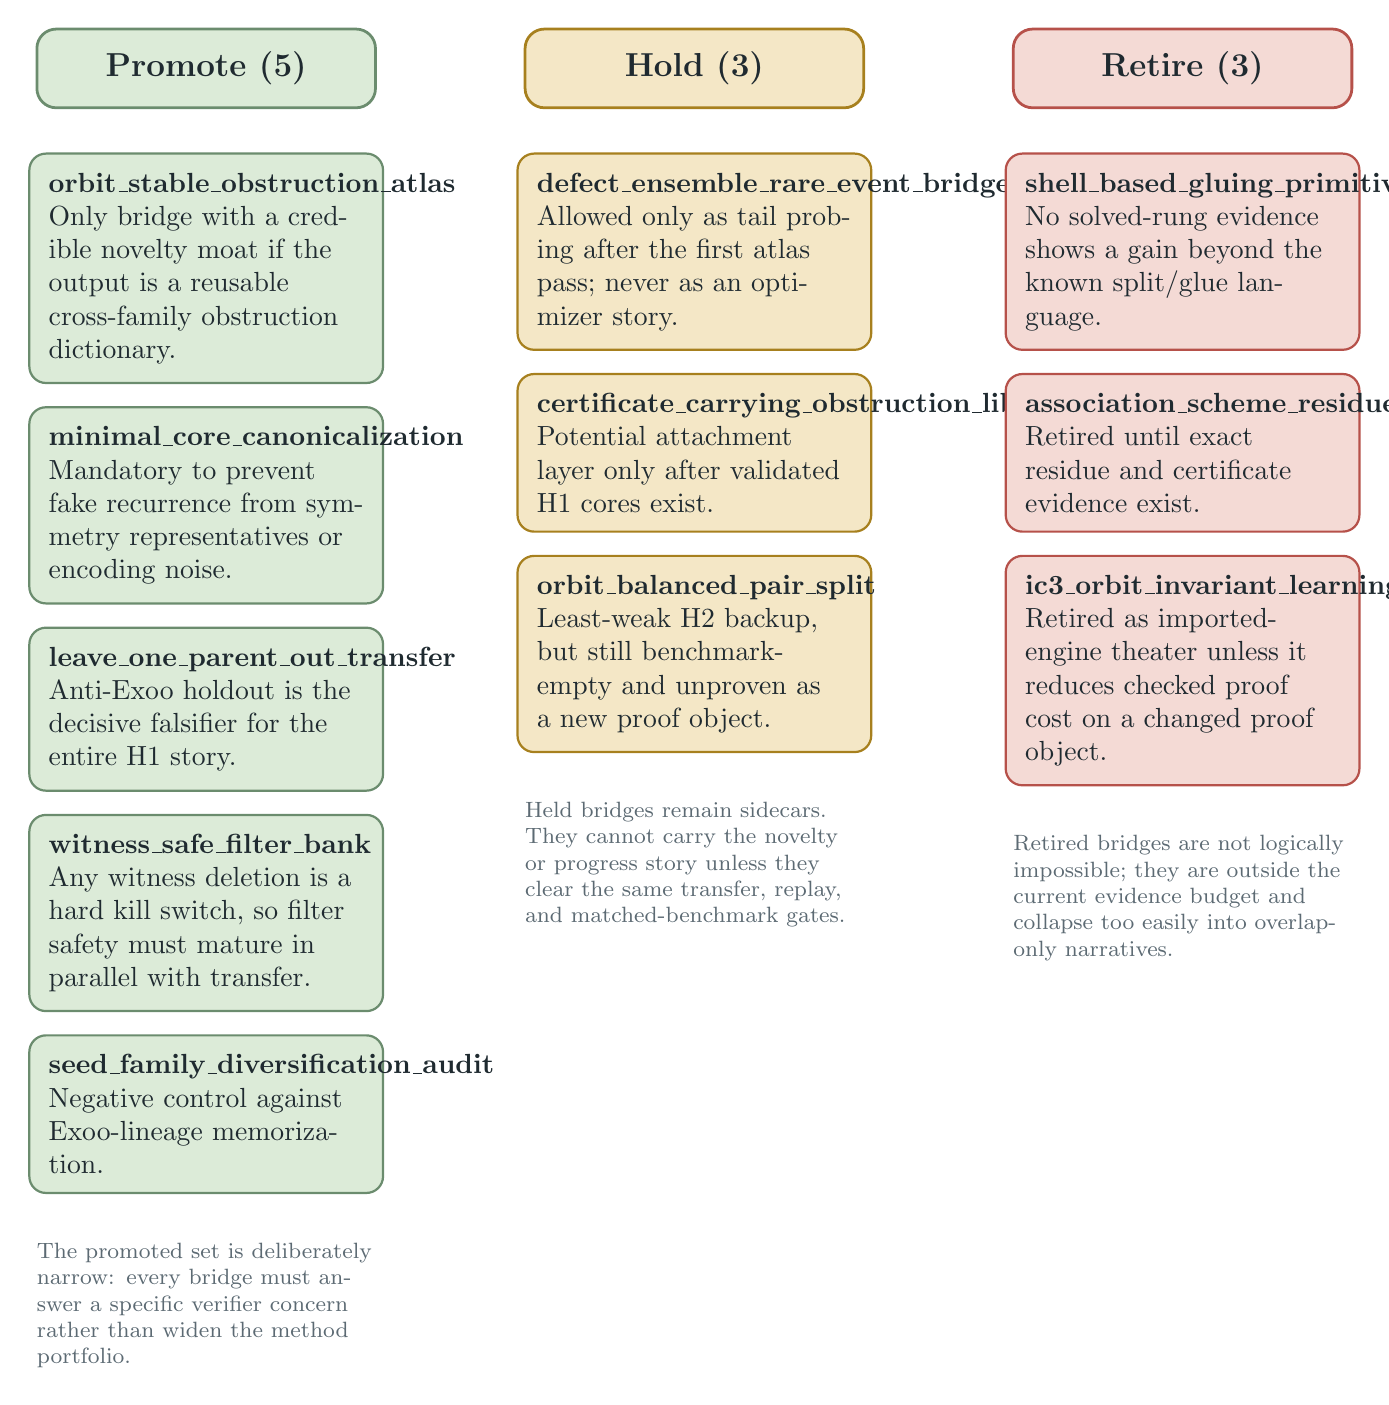
\begin{tikzpicture}[node distance=0.35cm and 0.7cm]
  \node[headercard, fill=softgreen, draw=sage] (phead) at (0,0) {Promote (5)};
  \node[headercard, fill=softgold, draw=gold!80!ink] (hhead) at (6.2,0) {Hold (3)};
  \node[headercard, fill=softred, draw=brick] (rhead) at (12.4,0) {Retire (3)};

  \node[promote, below=0.55cm of phead] (p1)
    {\textbf{orbit\_stable\_obstruction\_atlas}\\Only bridge with a credible novelty moat if the output is a reusable cross-family obstruction dictionary.};
  \node[promote, below=0.28cm of p1] (p2)
    {\textbf{minimal\_core\_canonicalization}\\Mandatory to prevent fake recurrence from symmetry representatives or encoding noise.};
  \node[promote, below=0.28cm of p2] (p3)
    {\textbf{leave\_one\_parent\_out\_transfer}\\Anti-Exoo holdout is the decisive falsifier for the entire H1 story.};
  \node[promote, below=0.28cm of p3] (p4)
    {\textbf{witness\_safe\_filter\_bank}\\Any witness deletion is a hard kill switch, so filter safety must mature in parallel with transfer.};
  \node[promote, below=0.28cm of p4] (p5)
    {\textbf{seed\_family\_diversification\_audit}\\Negative control against Exoo-lineage memorization.};

  \node[hold, below=0.55cm of hhead] (h1)
    {\textbf{defect\_ensemble\_rare\_event\_bridge}\\Allowed only as tail probing after the first atlas pass; never as an optimizer story.};
  \node[hold, below=0.28cm of h1] (h2)
    {\textbf{certificate\_carrying\_obstruction\_library}\\Potential attachment layer only after validated H1 cores exist.};
  \node[hold, below=0.28cm of h2] (h3)
    {\textbf{orbit\_balanced\_pair\_split}\\Least-weak H2 backup, but still benchmark-empty and unproven as a new proof object.};

  \node[retire, below=0.55cm of rhead] (r1)
    {\textbf{shell\_based\_gluing\_primitives}\\No solved-rung evidence shows a gain beyond the known split/glue language.};
  \node[retire, below=0.28cm of r1] (r2)
    {\textbf{association\_scheme\_residue\_screen}\\Retired until exact residue and certificate evidence exist.};
  \node[retire, below=0.28cm of r2] (r3)
    {\textbf{ic3\_orbit\_invariant\_learning}\\Retired as imported-engine theater unless it reduces checked proof cost on a changed proof object.};

  \node[ann, below=0.5cm of p5, text width=4.3cm]
    {The promoted set is deliberately narrow: every bridge must answer a specific verifier concern rather than widen the method portfolio.};
  \node[ann, below=0.5cm of h3, text width=4.3cm]
    {Held bridges remain sidecars. They cannot carry the novelty or progress story unless they clear the same transfer, replay, and matched-benchmark gates.};
  \node[ann, below=0.5cm of r3, text width=4.3cm]
    {Retired bridges are not logically impossible; they are outside the current evidence budget and collapse too easily into overlap-only narratives.};
\end{tikzpicture}
\end{document}
